\section{Introduction}
Graphical User Interface (GUI)~\citep{hong2024cogagent,cheng2024seeclick} agents have emerged as pivotal tools in automating interactions with digital devices, spanning from mobile applications~\citep{rawles2023androidinthewild,rawles2024androidworld,wang2024mobile,ye2025mobile} to desktop software~\citep{zhang2024ufo,qin2025ui,deng2023mind2web,xie2024osworld,cua2025,zheng2024gpt}. 
GUI grounding is a core capability of GUI agents, requiring the model to map natural-language instructions to specific interface elements on the screen, such as buttons, text fields, and icons~\citep{yang2024aria}. Early GUI grounding methods often rely on structured interface metadata, such as accessibility trees for mobile applications~\citep{zhang2025appagent}. Although such representations provide explicit descriptions of interface elements, they are limited in accessibility, often overly verbose, and may miss critical visual cues such as layout and icons.
These limitations have motivated a shift from metadata-based LLM grounding to screenshot-based multimodal large language models (MLLMs), which can directly reason over visual interfaces.

However, most existing MLLM-based GUI grounding methods~\citep{gou2024navigating,wu2024atlas,lin2024showui,xu2024aguvis} formulate the task in a coordinate-based manner, i.e., by directly predicting click coordinates as text tokens. This is an indirect formulation, since the model must compress fine-grained visual localization into textual coordinate generation. 
At the same time, recent evidence suggests that once GUI grounding is performed with MLLMs, useful query-visual grounding signals already emerge in their multimodal attention maps~\citep{xu2024attentiondrivenguigroundingleveraging}. 
This makes a more natural alternative possible: instead of generating coordinate tokens, one can perform coordinate-free GUI grounding by directly exploiting the MLLM's native attention as patch-level grounding cues, first identifying the relevant visual patches and then determining the specific click center within the selected region.

Recent efforts have begun to explore this direction. TAG~\citep{xu2024attentiondrivenguigroundingleveraging} leverages intrinsic query-visual attention in MLLMs, but aggregates attention maps from all query tokens in a vanilla manner, which is simple but often inaccurate. GUI-Actor~\citep{wu2025gui} also avoids direct coordinate generation, but introduces additional grounding modules instead of utilizing native attention and requires an extra adaptation stage. These limitations leave open an important question: can we directly specialize the \emph{intrinsic} multi-head attention of MLLMs for GUI grounding, without extra modules and without relying on impractical token-wise aggregation?

In this work, we propose \method{}, a coordinate-free GUI grounding framework that directly supervises the MLLM's multi-head self-attention (MHSA)~\citep{vaswani2017attention} with patch-wise grounding signals.
\method{} enables simple and fine-grained aggregation of patch-level attention vectors across all query tokens and all attention heads through two designs. First, we append a learnable $\texttt{<ANCHOR>}$ token after visual and query tokens, and use its attention over visual patches as a surrogate aggregator of query-visual interactions, thereby avoiding explicit token-wise aggregation. Second, we introduce a head-weighting mechanism based on \emph{visual-sink query tokens}: a small subset of query-side tokens selected from hidden-state similarity that reflects a strong query-visual connection. These tokens are used as proxies to identify attention heads that are more likely to encode grounding-relevant cross-modal correspondences, enabling more precise multi-head aggregation while minimally perturbing less grounding-relevant heads.

\begin{wrapfigure}[12]{r}{0.51\textwidth} 
\vspace{-1.3\baselineskip}
\centering
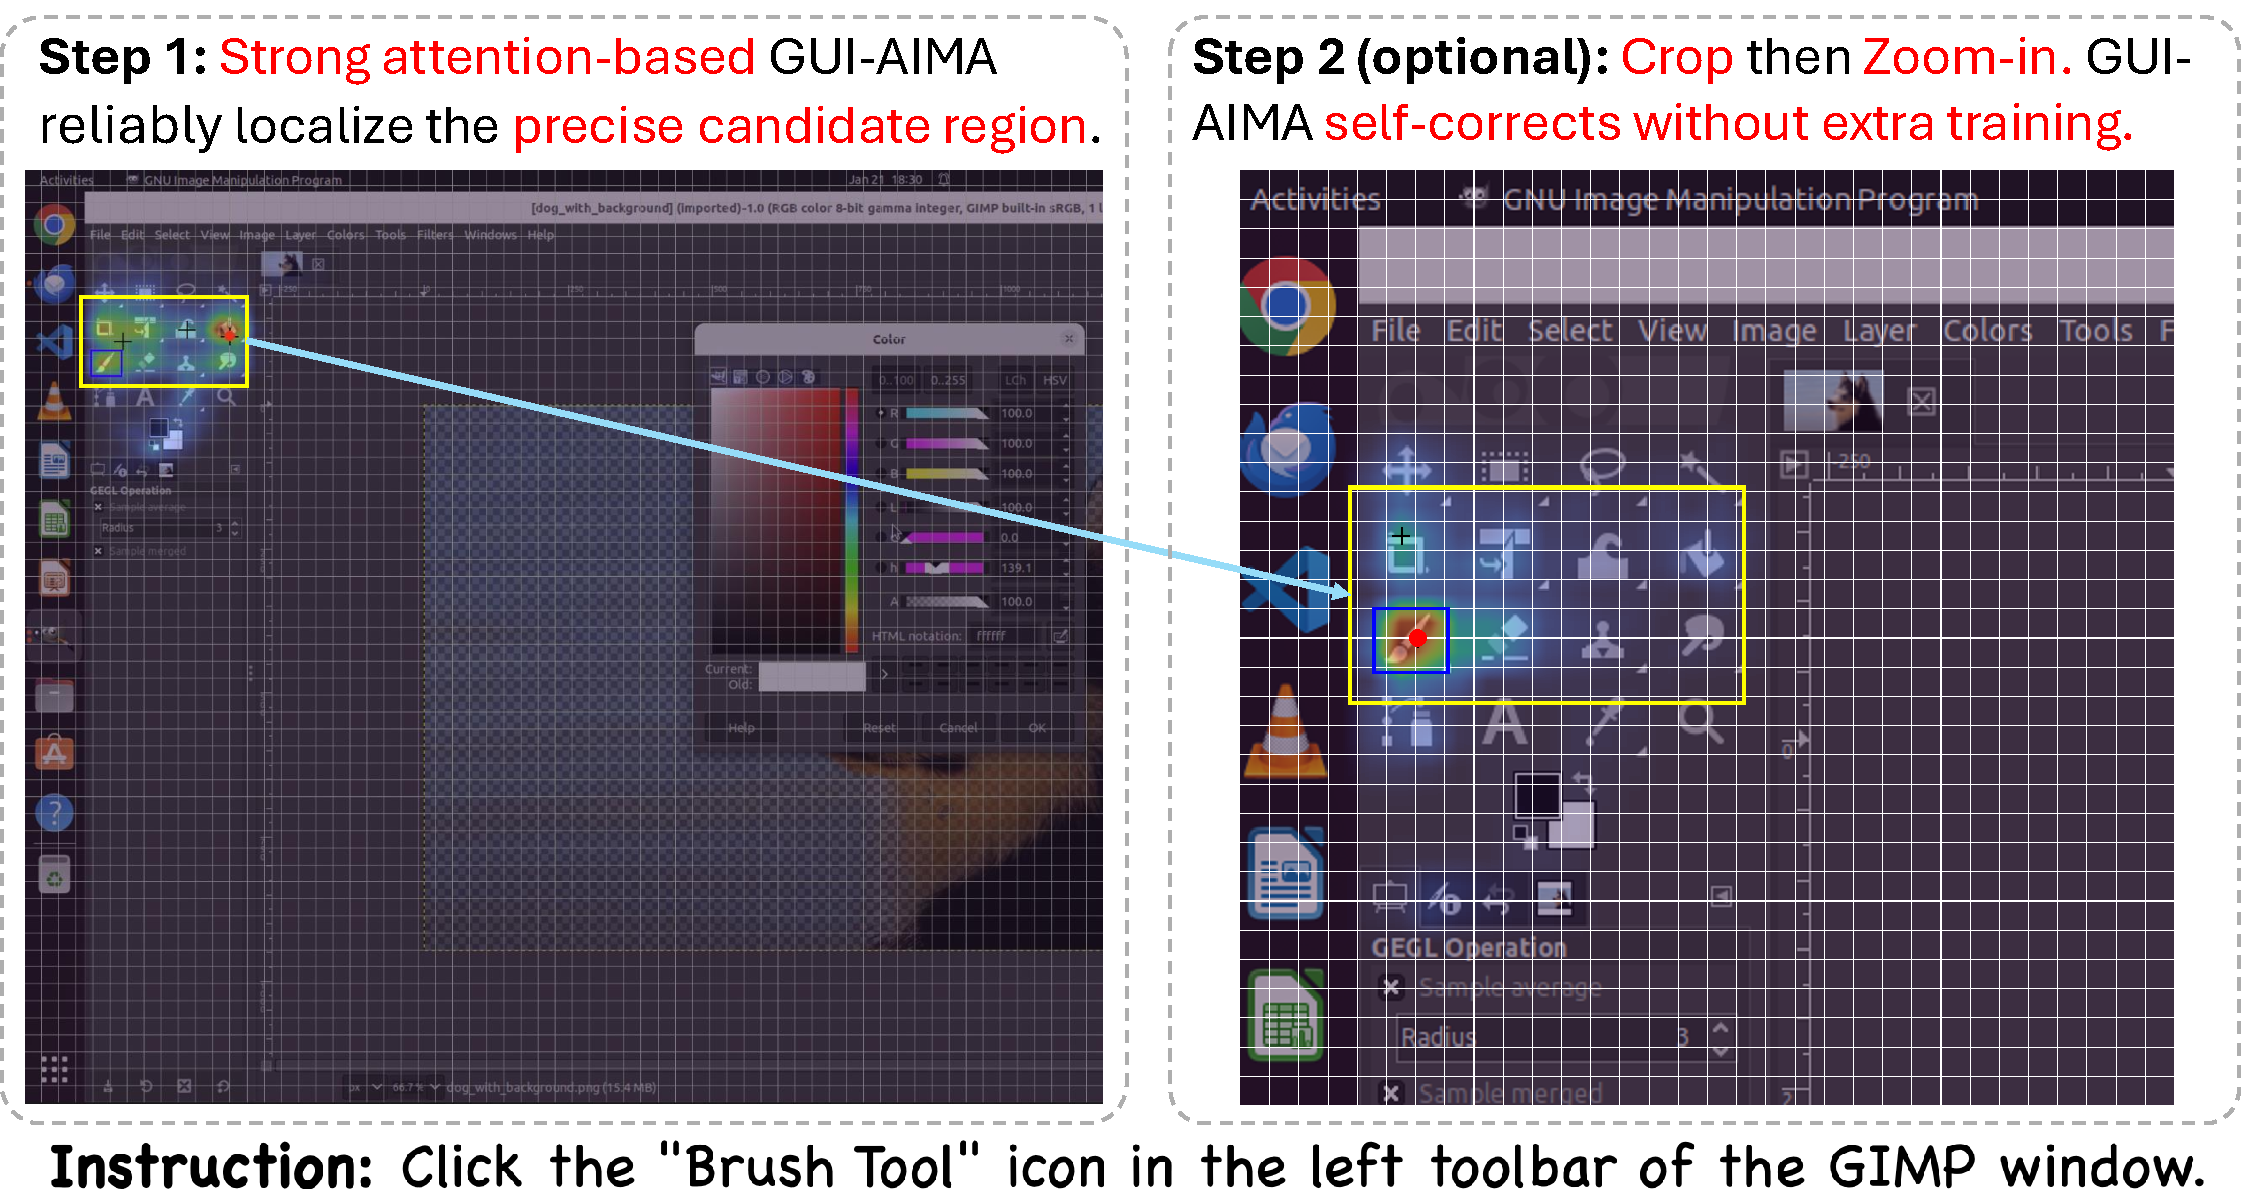
\includegraphics[width=\linewidth]{fig/two_step.pdf}
% \caption{An example of \method{} with two-step GUI grounding for hi-res screenshots.}
\vspace{-2em}
\caption{An example of \method{} with two-step GUI grounding for high resolution screenshots.}
% \vspace{1em}
% 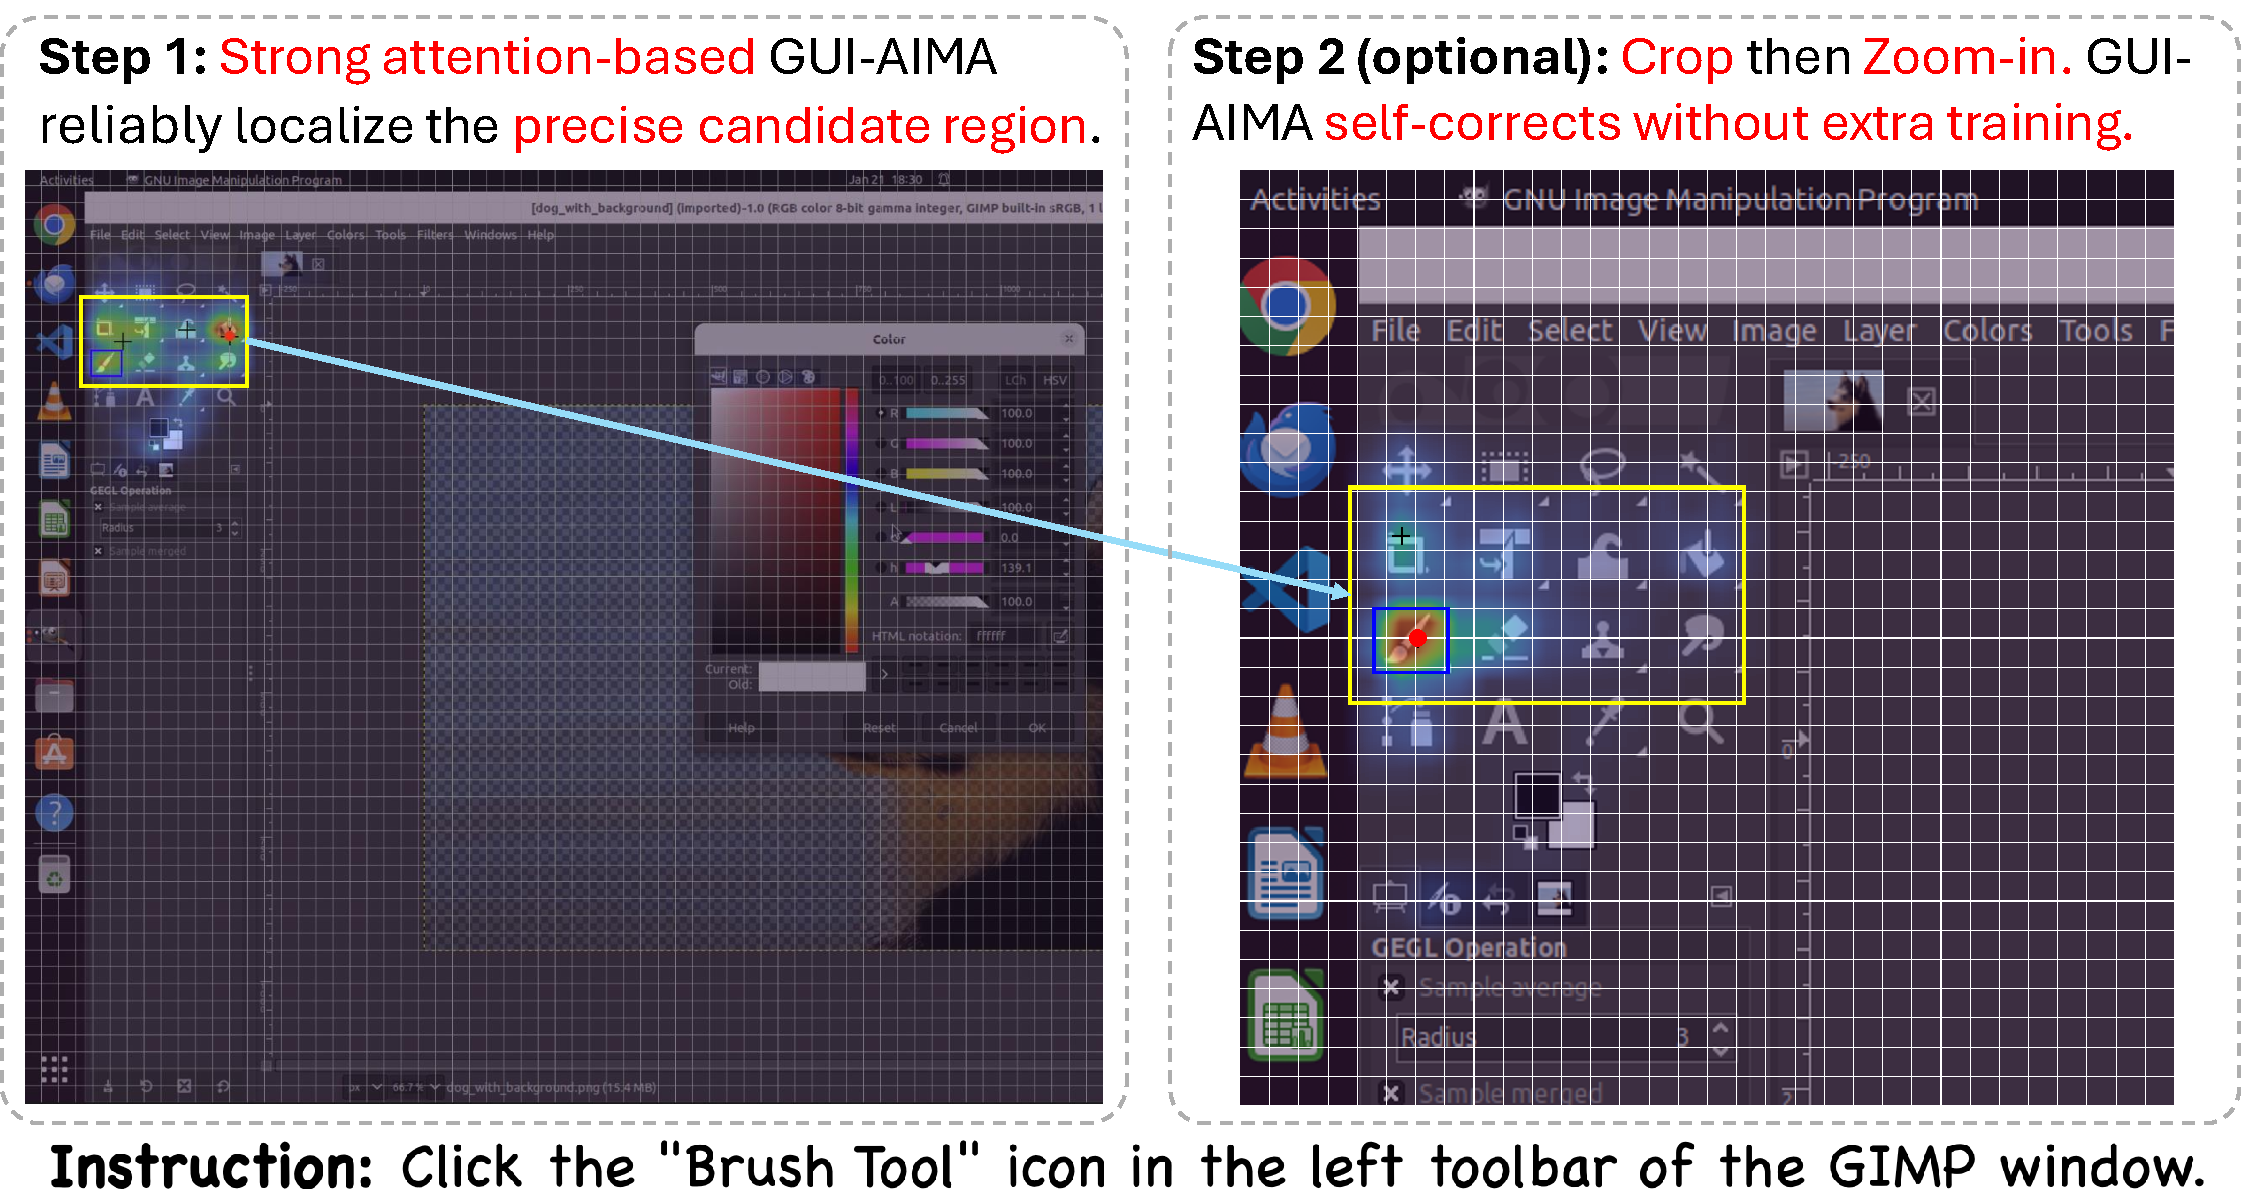
\includegraphics[width=\linewidth]{fig/two_step.pdf}
\label{fig:two_step}
\end{wrapfigure}
Built on this coordinate-free attention formulation, \method{} naturally supports practical improvements in both training and inference. We design an overlap- and distance-aware patch labeling that better matches click behavior. Moreover, because \method{} produces grounding from patch-level attention, it naturally enables a two-step zoom-in inference procedure for high-resolution screenshots: the model first localizes a coarse region, and then refines the prediction on a cropped view without additional training, as shown in \cref{fig:two_step}. This helps correct offset errors that commonly arise on dense, high-resolution interfaces.

\method{} is both effective and data-efficient. Under the ablation training setting, it improves ScreenSpot-Pro accuracy by 5.88\% over vanilla attention grounding (43.39\% over 37.51\%). With only one-stage fine-tuning on 101k screenshots without extra modules, \method{}-3B outperforms similarly sized models and remains competitive with substantially larger MLLM-based GUI grounding methods.

Overall, contributions of \method{} are as follows:
\begin{itemize}
    \item We propose \method{}, an attention-based, coordinate-free framework that directly leverages the intrinsic attention of MLLMs for GUI grounding, without introducing extra grounding modules.
    \item We develop a simple attention aggregation strategy that replaces impractical vanilla token-wise aggregation and a head-weighting mechanism that emphasizes grounding-relevant attention heads.
    \item We design a patch-wise labeling that better matches click behavior, together with a two-step zoom-in inference procedure for improved high-resolution localization.
    \item With only one-stage fine-tuning on 101k screenshots, \method{}-3B achieves strong data efficiency, outperforming similarly sized models and remaining competitive with substantially larger GUI grounding systems.
\end{itemize}